\chapter{Background}
\label{chap:background}

\emph{Draft Version}

%---
\section{Segmentation}

\subsection{Introduction}

Segmentation is a sub-field of image processing in which we try to partition an image into regions which correspond to interesting, or salient, features in the image. For instance, in medical image processing, we might try and segment a CT scan into regions which correspond to axial slices through major organs, e.g. the liver or a kidney. Segmentation is rarely useful on its own; rather, it tends to occur as a pre-processing step whose output (the partition of the image) is then used as input to later stages of an algorithm. An example usage is in the 3D visualization of organs, where the segmentation results for a series of slices can be used to identify which voxels in a volumetric dataset are contained within a given organ: a mesh can then be generated from this using any suitable algorithm from the visualization literature, e.g. \cite{cong05,lorensen87,wu03}.

Many different approaches are used to segment images. There is no `best' method which works well for every segmentation problem, so it is vital to select a method carefully based on the characteristics of the images under consideration. Since I will be dealing exclusively with \emph{medical} image segmentation of abdominal scans for the purposes of my thesis, I will only discuss techniques applicable in that domain in this review, but even with that restriction in place, there are several different image modalities (e.g. CT, MRI, US) which may be encountered and a large number of different segmentation methods in use \cite{pham00,varshney02}.

Each segmentation algorithm has its own characteristics (e.g. resilience to noise, connectedness of output, etc.), making it more or less suitable for a given problem. Some algorithms output region boundaries (contours) rather than an actual partition of the image \cite{kass88,lobregt95,xu98}: this may or may not be desirable in a given context (although it is worth noting that is often possible to subsequently convert between region-based and boundary-based representations). Furthermore, the degree of automation of the algorithms varies. At one end of the spectrum, images can be manually segmented by a radiologist: this generally gives excellent results (although they may not necessarily be entirely consistent between different radiologists) but requires more human interaction, although radiologists have got this down to a fine art. At the other extreme, we can try and develop algorithms which segment images automatically \cite{lee03, lin06, marcotegui05, meijster98, park03, soler01, touhami05, tsagaan02}: these reduce the burden on the human user, but it is rare that results are attained which are comparable with those which can be produced manually, not least because radiologists sometimes have to rely on anatomically-informed judgement to decide where the boundary of an object of interest lies and it is difficult to incorporate this expert knowledge into a computer program. That being said, some teams have achieved exceptionally good results in this area. Of particular note is the work done by Luc Soler's team in France \cite{soler01} which aims to delineate anatomical structures relevant to hepatic surgery. Clinical validation on over 30 patients has shown that their fully-automatic segmentation technique on 2mm-thick enhanced spiral abdominal CT scans generates results which are often actually \emph{better} than the manual segmentation produced by a radiologist.

In general, though, some degree of interactivity in segmentation procedures currently remains desirable, whether this merely involves allowing a radiologist to make adjustments to the output, or actually involves requesting user input to the algorithm itself (for example, a region growing algorithm might require seed points). There is a lot of overlap between the methods used for fully-automatic and semi-automatic segmentation --- in general, fully-automatic segmentation tends to focus (not surprisingly) on automating the difficult-to-automate aspects of semi-automatic algorithms --- so I will review approaches from both sub-fields in the following sections.

\subsection{Thresholding}

%TODO: \cite{kobashi95,seo05}

%In principle, thresholding segmentation methods are quite simple. The idea is to divide the pixels of the image into two (in the case of binary thresholding) or more (in the case of multithresholding) classes through the use of one or more dividing lines on the image histogram. For example, in an 8-bit image where the grey levels ranged from 0 (black) to 255 (white), we could decide that all pixels whose grey value was greater than 160 (say) represented the foreground of the image, and all other pixels represented the background.

In principle, thresholding segmentation methods are quite simple. The idea is to divide the pixels of the image into classes through the use of one or more dividing lines on the image histogram. Dividing the image into two classes is known as \emph{binary thresholding}; where more classes are used, we refer to the process as \emph{multi-thresholding}. As an example, we could use binary thresholding to divide an 8-bit image (with grey levels ranging from 0=black to 255=white) into two classes, one containing pixels greater than (say) 160, and representing the foreground of the image, and the other containing all the remaining pixels and representing the background.

The difficulty encountered in practice is how to determine the optimum threshold location(s). A misplaced threshold will cause an inaccurate segmentation, so choosing the location appropriately is essential. In our example above, choosing a threshold which was too high would mean that the foreground of the image would be \emph{undersegmented} (i.e. pixels which should be classified as being part of the foreground are incorrectly classified as background) and the background would be \emph{oversegmented} (the converse). Choosing too low a threshold would cause the opposite problem.

Owing to difficulties like this, applications are often designed so that thresholds can be chosen interactively by the user, but a great deal of work has also been done on automatically determining good threshold locations. As surveyed in \cite{sezgin04}, there are six types of approach to the problem in current use, including:

\begin{enumerate}

\item \emph{Histogram shape-based methods.} These use shape properties of the histogram to find a good threshold. For instance, Rosenfeld's histogram concavity method, cited in \cite{lee.c92}, works by examining the difference between a histogram and its convex hull. A grey level at which the the height difference between the histogram and its convex hull is greatest (i.e. a point of deepest concavity) is picked as the threshold value.

\item \emph{Clustering-based methods.} These try and group the grey level data into a given number of clusters (two in the case of binary thresholding). One example is the method of Ridler and Calvard \cite{ridler78}. Their idea was to take a grey-level image and produce an initial binary classification which makes the assumption that the object of interest is somewhere in the middle of the image and the corners of the image contain only background. The means of the pixels currently classified as background and object are calculated and the average of the two means is taken. The new value is then used to threshold the image and produce a new binary classification into background and object classes: it is assumed that this will be more accurate than the initial guess. Finally, the process is iterated until there is little or no change in the binary classification, and the last threshold in the iteration is chosen for use.

\item \emph{Entropy-based methods.} These are based on information theory and pick thresholds by (for example) trying to maximise the information content in the thresholded image. As described in \cite{wong89}, the simplest possible method looks at two probabilities, $F(T)$ and $F^*(T) = 1 - F(T)$, each parameterised in terms of a threshold, $T$. The first, $F(T)$, gives us the probability of a given pixel having a grey value less than or equal to the threshold, and the second, $F^*(T)$, gives us the probability of the value being greater than it. The information content in the thresholded image is given by
%
\[
H(T) = -F(T) \log_2 F(T) - F^*(T) \log_2 F^*(T)
\]
%
and attains a maximum when $F(T) = 0.5$. This is equivalent to saying that in the absence of any other knowledge, the maximum entropy principle tells us that the information contained in the thresholded image is maximised by picking a threshold which classifies half the pixels as background and half as foreground. This makes intuitive sense, but is too simplistic an approach for the majority of applications. Better alternatives have been developed, but are beyond the scope of this report.

%\item \emph{Object attribute-based methods.}

%\item \emph{Spatial methods.}

%\item \emph{Local / adaptive methods.}

\end{enumerate}

\noindent In spite of the large amount of work done on thresholding, however, it has some significant downsides when used on its own to process medical images:

\begin{itemize}

\item It divides the image into two or more groups of pixels, based on their grey values, but there is no guarantee (or even an expectation) that any of these groups will be contiguous in the image. For instance, trying to segment a kidney from a CT scan by bounding it between two grey value thresholds might also result in inadvertently segmenting blood vessels across the image as well (their grey levels are quite similar to those of the kidneys). Not only are these blood vessels not part of the kidney, they are actually physically separated from it in the image! (It is also worth noting that trying to segment a kidney will generally result in segmenting both of them at once, since their grey level ranges are the same. This sort of problem can be overcome by specifying the side of the body in which we're interested.)

\item It is by no means the case that acceptable threshold locations always exist. If the grey value ranges of different objects of interest significantly overlap, it may be impossible to separate them using thresholding alone.

\end{itemize}

%For reasons like this, I believe that thresholding is not the most appropriate choice of method for my work. However, I have found a use for it when trying to quantify the extent of necrosis in a tumour (see Chapter~\ref{chapter:existingwork}).% Whilst it is true that thresholding can be made to produce reasonable results (e.g. \cite{kobashi95}), I feel that there are other algorithms which

These limitations can often be overcome by combining thresholding with other techniques. For instance, the results of thresholding often have gaps in them, which can sometimes be filled in by carefully applying various morphological operators (e.g. morphological opening and closing). Luc Soler's team \cite{soler01} made use of thresholding (as one technique among many) and achieved excellent automatic segmentation results for the liver. However, they did not use thresholding on its own. For instance, they segmented bones by thresholding for bright areas and then keeping only those which were near to the fat tissue (which had already been segmented). Simple thresholding alone would have been insufficient for the task, since structures such as the aorta also appeared bright on the contrast-enhanced images.

%Whilst thresholding has its limitations, it has been nevertheless been successfully incorporated into more general segmentation algorithms, sometimes with spectacularly good results. The work of Luc Soler's team \cite{soler01}, as previously commented on, is particularly noteworthy in this regard. One example of how they use thresholding to achieve good results is when they are segmenting bones. A simple thresholding operation would fail, since the contrast agent used when the scans were taken causes structures such as the aorta to appear bright. Instead, they isolate the fat tissue and define the bones as being bright structures close to that. They also post-process their thresholding operations with morphological operators to fill in any unwanted gaps.

\subsection{Region Growing}

%TODO: \cite{lin06,pohle01}

Region growing methods for segmentation essentially work as follows. First, an initial seed point is chosen for a feature of interest. Then, the region is `grown' by iteratively considering all points which are adjacent to the region and adding any which satisfy certain criteria. For example, we could choose to add adjacent pixels whose grey value differs from that of their neighbour in the region by less than a certain amount. Alternatively, we could try and add adjacent pixels which preserve the homogeneity of the entire region (for some suitable definition of homogeneity). A basic region growing algorithm can be implemented straightforwardly using a queue. Starting from a queue containing only the initial seed point, we repeatedly pop the pixel at the front of the queue, consider its non-region neighbours for addition to the region, and push any which satisfy the requisite criteria onto the end of the queue. The process terminates when the queue empties.

The key issues when implementing region growing are how to choose the seed point, how to formulate the criteria specifying which points to add to the region, and how to decide when the process should terminate. For automated segmentation methods, how to choose the seed point is of fundamental importance; semi-automated algorithms can focus exclusively on the latter two problems, relying instead on the user to interactively specify an initial seed.

As mentioned above, one of the simplest approaches to region growing is to add adjacent pixels which are within a certain fixed threshold value of their neighbour in the region. Practical region growing methods, however, such as \cite{lin06,pohle01}, tend instead to use \emph{adaptive} region growing, whereby the criterion varies to take account of the area around the pixel under consideration. In \cite{lin06}, for example, the approach taken is as follows. After locating an initial seed point $(s_x, s_y)$, a $7 \times 7$ mesh is placed over it and the maximum and minimum pixel intensities within the mesh, $M(s_x, s_y)$ and $m(s_x, s_y)$ are determined. From these, a contrast range $t_0 = M(s_x, s_y) - m(s_x, s_y)$ is calculated and recorded. Next, for each pixel $(x,y)$ under consideration for addition to the region, values $M(x,y)$ and $m(x,y)$ are similarly calculated, and a local value $\theta_{\rm local} = (M(x,y) + m(x,y)) / 2$ is determined. The region growing criterion is then formulated as $|f(x,y) - \theta_{\rm local}| \le t_0$, i.e. we add an adjacent pixel $(x,y)$ to the region if the absolute difference between its grey value $f(x,y)$ and the midpoint of the contrast range of the $7 \times 7$ mesh surrounding it is less than the contrast range of the $7 \times 7$ mesh centred on the initial seed point. The region growing is specified to stop when this absolute difference is greater than a certain threshold, implying that the area surrounding a given pixel is not homogeneous.

The advantages of region growing methods are that the resultant region is guaranteed to be connected in the image (unlike with thresholding) and that they are, on the whole, fairly easy to implement. However, from the point of view of automatic segmentation, they present difficulties, because choosing an initial seed point is in general a non-trivial problem. The usual approach taken for automatic seed point selection is to rely on statistical data about where the features of interest (e.g. organs) usually lie in the body. For instance, the approach in \cite{lin06} is to search for suitable seed points in two elliptical regions on each side of the body, one for each kidney. This works quite well, but doesn't seem as if it would be that robust if tested on unusual cases.

Whilst region growing algorithms are guaranteed to produce a connected result, the region may still have holes in the middle of it. Whilst this may be desirable if we really are trying to segment a torus-shaped feature, on the whole we need to post-process the region growing results to remove these holes. Common techniques for doing this include morphological closing, etc.

\subsection{Approaches from Mathematical Morphology}

In the words of some of its practitioners\footnotemark{}, the field of mathematical morphology espouses a `non-linear approach to image processing'. Its interesting techniques include dilation, erosion, and morphological opening and closing, but our emphasis in this report will be on one particularly useful morphological technique for image segmentation: the watershed transform.

\footnotetext{The Centre for Mathematical Morphology at the Ecole des Mines de Paris.}

\subsubsection*{The Watershed Transform: Techniques}

%TODO: \cite{bieniek00,meijster98,osma-ruiz06,rambabu07,stoev00}

\emph{Note: I have written an article on the watershed transform for ACCU's Overload journal, which appears as Appendix~\ref{chapter:watershed} in this report. For that reason, I plan to give only a limited presentation of the technique here. Readers are referred to the appendix for more information.}

The idea of the watershed transform is to view an image as a landscape and divide it up into valleys. Each valley in the landscape will correspond to a region in the segmentation result. We don't perform the transform on the actual image to be segmented, since its valleys may not correspond to the features we're interested in. Instead, we take the initial image and try and generate a derived image from it in which the valleys correspond to our features of interest: in the case of medical images, this often involves something similar to taking the gradient of the initial image, since organs tend to look fairly homogeneous on scans (and thus the magnitude of the gradient within them is low). The derived image then becomes the input to the watershed transform itself.

In terms of implementation, the watershed transform can be viewed in one of two different ways:

\begin{enumerate}

\item \emph{A flooding/immersion process}. Imagine poking holes in the local minima of the landscape and then lowering the landscape vertically into a lake. As the landscape is lowered, water will seep through the holes and catchment basins will form in each of the valleys of the image. As the water continues to rise, some of the catchment basins will meet: at this point, we add dams, or watersheds, to keep them apart, and continue lowering the landscape. At the end of the process, the dams we added will act as dividing lines between the valleys, thus segmenting the underlying image into regions.

\item \emph{A rainfall process}. Imagine dropping a raindrop at each point in the landscape. Assuming the image has no (non-minimal) plateaux (flat regions), the drop will run downhill, via a path of steepest descent, until it ends up in a local minimum. (There are ways of dealing with non-minimal plateaux, e.g. the method described in the appendix.) The point at which it started will be associated with this local minimum (it will be called part of the minimum's catchment basin) and the process will continue until all the points in the landscape have been processed. The result will be a region-based partition of the landscape (and hence the underlying image) into catchment basins, one per local minimum.

\end{enumerate}

These two alternative ways of viewing the process have led to two different classes of techniques. In particular, \cite{bieniek00} and \cite{rambabu07} are examples of the former approach, and examples of the latter can be found in \cite{meijster98,osma-ruiz06,stoev00}. It is worth noting that the various definitions are not always exactly equivalent. For example, some approaches generate results containing watershed lines, whilst others generate only regions. Also, rainfalling approaches don't generally give identical results to their immersion-based counterparts. It is thus important to choose an appropriate method with care.

\subsubsection*{The Watershed Transform: Pre-Processing}

%TODO: \cite{ancin95}

The biggest problem with the watershed transform as a segmentation approach is that it is overly affected by spurious local minima in the landscape. This leads to massive over-segmentation of the image. To explain the problem, consider an analogy. If we try and divide a dimpled landscape into valleys, counting each dimple (small hollow) in the landscape as a valley, then we will end up with vast numbers of `irrelevant' valleys at the end of the process, obscuring the more significant valleys we are trying to find: this is essentially the problem faced by the watershed transform. The `dimples' in an image can be caused by things like noise, but even in the absence of image artifacts, there will usually be valleys corresponding to features in which we have no interest. We need a way of separating the wheat from the chaff.

To overcome this difficulty, various approaches have been suggested in the literature. The effects of less prominent noise can be mitigated to an extent by smoothing the image, although care must be taken not to blur the edges in the image when doing this. Another approach \cite{ancin95} is to suppress some of the irrelevant contours in the gradient image by determining the connected components of the gradient image and removing (by setting the pixels of the component to zero) all those whose size is less than a threshold (e.g. the perimeter of the smallest object of interest).

One technique which works quite well in practice is to apply spatially-variant smoothing to the image: instead of smoothing uniformly over the entire image, the idea is to smooth less in areas where we think there may be edges. This is the idea behind non-linear diffusion filters \cite{perona90}. (In Chapter~\ref{chapter:existingwork}, I describe another approach based on similar principles.)

\subsubsection*{The Watershed Transform: Post-Processing}

%TODO: \cite{beucher01,patino05,marcotegui05,wegner95}, \cite{najman96} (mention correction paper)

The approaches described so far try to pre-process an image (or its gradient image) to reduce watershed over-segmentation. Post-processing the watershed results is also possible, and in general a combination of both techniques tends to be employed.

The general idea of watershed post-processing is to try and merge the large number of generated regions together in a way that generates larger regions corresponding to our objects of interest. Attempts can be made to group together similar regions using fuzzy relations, e.g. \cite{patino05}.

The idea of region-merging can also be used to create partition hierarchies, intuitively corresponding to a series of segmentations of an image at different scales. For example, the waterfall algorithm \cite{beucher01,marcotegui05} merges regions by iteratively running a watershed-from-markers algorithm on the region adjacency graph of the watershed result. (Note that I have described it in much more detail in Appendix~\ref{chapter:waterfall}.) This is particularly useful when trying to pick out organs of different sizes. A similar approach is described in \cite{wegner95}.

The type of hierarchy generated by the waterfall algorithm is by no means the only possible hierarchy, and indeed it may converge (to a single region) too fast for some applications. Alternative hierarchies are also possible, e.g. ones based on the saliency of contours in the watershed results \cite{najman96}.\footnotemark{}

\footnotetext{Whilst this is generally a good paper, it is worth noting that it contained an error which had to be corrected later in a comment \cite{lemarechal98}. An improved correction was then published by one of the original authors \cite{schmitt98}. All three should be read together to avoid confusion.}

%\subsubsection*{The Watershed Transform: Applications}

%TODO: \cite{bueno01,grau04}, mention \cite{najman95} in the context of registration

\subsection{Deformable Models}

%Model fitting methods, as their name suggests, attempt to fit a model of the features under consideration to the actual data available. They essentially make use of \emph{a priori} anatomical knowledge at an early stage of the segmentation process to improve the generated results. The actual model used can take a variety of different forms, ranging from deformable models, whereby the model is represented explicitly (perhaps as a contour on the image), to implicit model representations such as probabilistic atlases and neural networks. I will briefly survey each of these methods in the subsections which follow.

%As their name suggests, deformable models methods work by taking an initial model of the features under consideration and deforming it to fit the actual data available. The initialisation of the model is generally based on \emph{a priori} anatomical knowledge. As observed in \cite{suri02}, there are two basic types of deformable model, namely \emph{parametric} and \emph{geometric}. Geometric deformable models have been developed more recently than their parametric counterparts, but both types see a lot of use. The most well-known examples of the two types are snakes and level sets, which will be discussed in detail in the following two subsections.

As their name suggests, deformable models methods work by taking an initial model of the features under consideration and deforming it to fit the actual data available. The initialisation of the model is generally based on \emph{a priori} anatomical knowledge. The model itself can be represented in a variety of ways, and these ways correspond to a number of different approaches to the problem. For example, the snakes method, which we will see shortly, represents the model as a parametrically-defined spline, and is hence referred to as an example of a parametric deformable model (it is sometimes also referred to as an explicit deformable model). In contrast, level sets represent the model \emph{implicitly} and are an example of implicit deformable models. Implicit deformable models were developed more recently than their parametric counterparts, but both types see a lot of use.

\subsubsection{Snakes}

%TODO: \cite{cohen91,kass88,lobregt95,xu98}

As originally defined by Kass, Witkin and Terzopoulos in \cite{kass88}, ``A snake is an energy-minimizing spline guided by external constraint forces and influenced by image forces that pull it toward features such as lines and edges.''

Essentially, the idea works as follows. We represent the position of the snake, in terms of a spline parameter $s$, as $\mathbf{v}(s) = (x(s),y(s))$, and define an \emph{energy functional}, $E_{snake}^*$, as
%
\[
E_{snake}^* = \int_0^1 E_{int}(\mathbf{v}(s)) + E_{image}(\mathbf{v}(s)) + E_{con}(\mathbf{v}(s)) \; ds.
\]
%
The three terms in the summation are \emph{internal} energy, which tries to limit the curvature of the snake, \emph{image} energy, which tries to attract the snake towards features in the image such as lines and edges, and \emph{constraint} energy, which allows the user to apply constraints to influence the result of the segmentation. The snake algorithm as a whole attempts to find a spline minimising $E_{snake}^*$.

The original snakes paper describes a continuous model, but more recent research \cite{lobregt95,miller90b,miller90a} has seen the development of discrete models as well. The model described by Lobregt and Viergever in \cite{lobregt95}, called a \emph{discrete dynamic contour model}, is particularly interesting, both because it is intuitively easy to understand, and because it links in with my previous work. It is thus worth describing in more detail.

Rather than relying on ideas of energy-minimization, Lobregt and Viergever model snakes using a force-based physical simulation (note that this ties in well with my earlier work on physical simulations of long hair \cite{gvc08}). In their approach, a snake is a set of vertices connected by edges. At each time-step, various forces are applied to each vertex, which gradually \emph{deform} the snake towards the desired result. The results of this approach will depend to an extent on the lengths of the edges joining the vertices: if an edge is too long, important image features may pass through the gaps between vertices; if it is too short, the snake may become overly fixated on small details, not to mention the speed of the process being adversely affected. For this reason, after each deformation step, the snake is \emph{resampled} (by adding or removing vertices where necessary) to keep the edge lengths within certain limits.

The forces applied to each vertex closely mimic the energy terms in the original snakes paper. The force $\mathbf{f_i}$ applied to vertex $i$ is defined as the weighted sum
%
\[
\mathbf{f_i} = w_{ex}\mathbf{f_{ex,r_i}} + w_{in}\mathbf{f_{in,i}} + \underbrace{w_{damp}}_{< \; 0}\mathbf{v_i},
\]
%
where $\mathbf{f_{ex,r_i}}$ is an \emph{external} force term corresponding to the image and constraint terms from the original formulation, $\mathbf{f_{in,i}}$ is an \emph{internal} force term corresponding to the original internal term, and the remaining term is a new addition used to apply damping to try and bring the simulation to rest. (The real numbers $w_{ex}$, $w_{in}$ and $w_{damp}$ specify the weights to be given to each of these three factors. The paper tended to set all three of these to $0.5$: apparently this was derived empirically.)

It is important to mention that the method relies on quite a close initialisation (i.e.\ image features have quite a short capture range). In \cite{ree05}, this problem is circumvented by peforming a watershed-from-markers segmentation and using the result of that to initialise the snake. Another alternative, referred to there, is to try and add additional external forces to solve the problem: in particular, some success has been had with \emph{balloon forces} \cite{cohen91} and \emph{gradient vector flow} \cite{xu98}.

Problems of this kind with snakes methods have led to a great deal of interest in level sets as an alternative, although snakes also remain popular as a well-established and far simpler alternative. They also have the advantage that they can represent open structures as well as closed ones.

\subsubsection{Level Sets}

%TODO: \cite{sorlie05}

Level sets are to snakes what implicit representations of functions are to parametric ones. As an initial introduction, consider the alternative representations of a circle of radius $r$, centred at the origin. An implicit representation could be
%
\[
x^2 + y^2 = r^2,
\]
%
whereas a parametric representation in terms of an angle $\theta$ could be
%
\begin{eqnarray*}
x & = & \cos \theta \\
y & = & \sin \theta.
\end{eqnarray*}
%
Now, consider a more general form of the above. Instead of thinking about circles, consider the function $\phi(x,y) = x^2 + y^2$, which defines a scalar field over $\mathbb{R}^2$. For any value $k > 0$, the equation $\phi(x,y) = k$ defines a circle in the x-y plane: we will refer to each of these circles as an \emph{isosurface} of $\phi$, because each of them is the surface (curve) of all the points at which $\phi$ takes a particular value\footnotemark{}.

\footnotetext{\emph{Iso} means `equal' in Greek, so here we are talking about the surface containing all the points with the same $\phi$ value.}

Note what happens if we change $\phi$. If we redefine it as $\phi(x,y) = x^3 + y^3$, the isosurfaces change from being circles to hypercircles. This is a key idea: by changing the function $\phi$, we can move the isosurfaces of $\phi$ around, \emph{without having to represent them explicitly}. This is the insight behind level sets: we represent the contour we're interested in as an isosurface of some function $\phi$, then modify $\phi$ to modify the contour. Instead of using simple functions like $x^2 + y^2$ for our $\phi$, we can think of a general function $\phi: U \to \mathbb{R}$, where $U \subset \mathbb{R}^2$.

In practice, to represent contour changes over time, we make $\phi$ a function of time as well, giving us $\phi(\mathbf{x},t): U \times \mathbb{R}^+ \to \mathbb{R}$. We then set this equal to some constant $k$ to actually specify which isosurface of $\phi$ we're interested in.

Consider a simple example, that of a circle, centred at the origin, which gradually expands outwards as the time increases (see Figure~\ref{fig:levelsets-circle}).

%---
\stufigex{height=7cm}{background/levelsets-circle.png}{A simple circular contour which gradually expands over time}{fig:levelsets-circle}{H}
%---

In particular, suppose its radius is $t$ at time $t$. We represent this as:
%
\[
\phi((x,y), t) = \frac{x^2 + y^2}{t^2} = 1 = k
\]
%

For a more complicated example, consider gradually changing the circle into an ellipse over time (see Figure~\ref{fig:levelsets-ellipse}).

%---
\stufigex{height=7cm}{background/levelsets-ellipse.png}{An example of a contour which changes its shape over time}{fig:levelsets-ellipse}{H}
%---

This could be achieved by writing the following:
%
\[
\phi((x,y), t) = \left(\frac{x}{t}\right)^2 + y^2 = 1 = k
\]
%

In practice, we are almost never able to give an explicit function for $\phi$: the simple examples above notwithstanding, it's just not possible for real-world applications. Instead, we discretise the process by specifying initial values for $\phi$ at points on a discrete grid, then derive a partial differential equation for $\phi$ and solve it numerically to modify the contour over time. The PDE in question can be found by taking the total derivative of
%
\[
\phi(\mathbf{x}, t) = k,
\]
%
giving us
%
\[
\pd{\phi}{t} = -\nabla\phi \cdot \mathbf{v},
\]
%
where $\mathbf{v} = \pdnf{\mathbf{x}}{t}$. By making $\mathbf{v}$ a function of the position of $\mathbf{x}$ and the geometry of the surface (which it turns out can be represented by the differential structure of $\phi$), we can control how we want the contour to evolve over time.

How to numerically solve the above equation is beyond the scope of this report, but before moving on, I would like to look at a concrete example of the method on a discrete grid, to illustrate some of its advantages. Consider the discrete grid of $\phi$ values in Figure~\ref{fig:levelsets-discrete1}(a). The marked points form an isosurface of $\phi$, specifically the $k = 4$ isosurface. This is entirely analogous to the examples above, but on a discrete grid instead of in a continous space. By changing the grid values, as in Figure~\ref{fig:levelsets-discrete1}(b), we can move the isosurface however we wish.

%---
\begin{figure}[H]
\begin{center}
	\subfigure[]{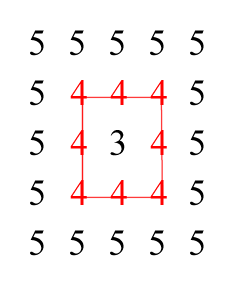
\includegraphics[height=5cm]{background/levelsets-discrete1a.png}}%
	\hspace{4mm}%
	\subfigure[]{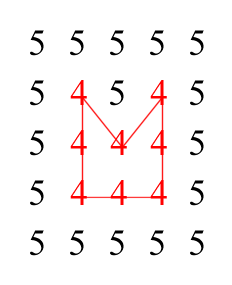
\includegraphics[height=5cm]{background/levelsets-discrete1b.png}}
\end{center}
\caption{An example of level sets on a discrete grid}
\label{fig:levelsets-discrete1}
\end{figure}
%---

Now, consider the further example shown in Figure~\ref{fig:levelsets-discrete2}(a). Here the situation seems more complicated, in that the points on the $k = 4$ isosurface are not all connected to each other. This is actually an advantage of the level set method, however. By representing the surface implicitly, we can model surfaces with multiple connected components without having to do any additional work. Indeed, the number of components can evolve over time: in Figure~\ref{fig:levelsets-discrete2}(b), we see that the two components can be joined by simply changing the value of $\phi$ at one of the grid points to $5$.

%---
\begin{figure}[H]
\begin{center}
	\subfigure[]{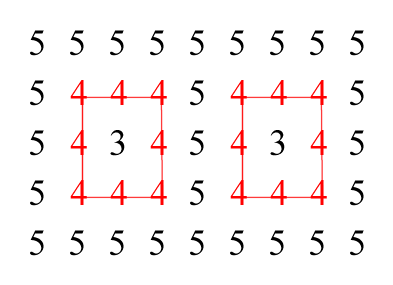
\includegraphics[height=5cm]{background/levelsets-discrete2a.png}}%
	\hspace{4mm}%
	\subfigure[]{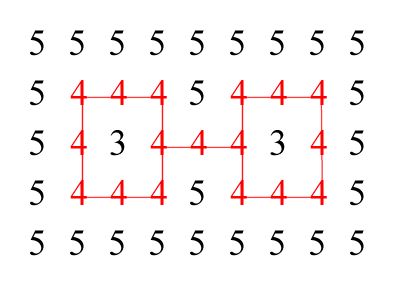
\includegraphics[height=5cm]{background/levelsets-discrete2b.png}}
\end{center}
\caption{An example with more than one connected component}
\label{fig:levelsets-discrete2}
\end{figure}
%---

One final advantage of level sets worth mentioning is that the method works equally well in 3D, although the extra processing involved means that clever numerical techniques are required. The details of how these work are beyond the scope of this report but, as an example, one method (the narrow-band technique) basically restricts numerical calculations to a narrow region around the isosurface we're particularly interested in. The insight is that solving the PDE over the whole domain is only necessary if we're interested in solving for the entire family of isosurfaces associated with $\phi$: often we're only looking at a single isosurface, so the extra computations aren't necessary. For more details, take a look at \cite{yoo04}.

\subsubsection{Other Deformable Models}

%TODO: \cite{jalba04,rao05,tsagaan02}

Other notable parametric deformable models in existence include the contribution of Tsagaan et al. \cite{tsagaan02}, who used a NURBS-based model of a kidney and deformed it by minimising an energy function. Their results seem good in some cases, but differ markedly from the manually segmented results in others.

Parametric and implicit models are not the only types of deformable model in use, however. In particular, \cite{jalba04} uses a deformable model based on charged particles to achieve some interesting automatic segmentation results. Here, the model is represented as a set of charged particles under the influence of an electrostatic field. The authors' work in this area is still ongoing. Yet another deformable model can be found in \cite{pizer03}, in which the authors' make use of a medial representation known as m-reps.

\subsection{Learning Methods}

Learning segmentation methods generally start with a training phase, in which a large number of scans are taken and used to construct some variety of model, which encodes information that can be used to segment subsequent scans. Two different types of learning method will be discussed in the following subsections.

\subsubsection{Atlas-Based Approaches}

%TODO: \cite{park03,zhou05}

Atlas-based methods start by constructing an atlas, or reference segmentation, from a set of training data. For instance, in \cite{park03}, a probabilistic atlas was constructed by registering (aligning) the manually segmented volumes of 31 patients onto that of a carefully chosen reference patient (thus the data came from 32 patients in all). The atlas was represented as a 3D grid of vector values, where the components of each vector corresponded to the organs under consideration, and the values of the components indicated the fractional percentage of registered data sets in which the point was labelled as the given organ. As an example, if we were considering the liver and the two kidneys, the vector $(0.4, 0.6, 0)^T$ at a point could indicate that the point was inside the liver in 40\% of the data sets and inside the right kidney in 60\% of them.

After constructing such an atlas, new sets of data can be segmented by registering them onto it. In \cite{park03}, they use a \emph{maximum a posteriori} (MAP) approach after registration to find the segmentation result which best explains the observed data. The important point here is that the segmentation result is based on both the data for the individual patient and the information encoded in the atlas. The atlas provides the prior probabilities at each voxel, and these are refined in light of the actual patient data.

To use the notation in \cite{park03}, we denote the segmentation result field as $\mathbf{X}$, the field of observed data for the individual patient as $\mathbf{Y}$, and the probabilistic atlas as $\mathbf{A}$. Each of these represents a volume of $N$ voxels, indexed linearly (in some order) from $1$ to $N$. So for instance, a particular segmentation result could be given by $\mathbf{x} = (x_1, x_2, \ldots, x_N)$. Our aim is to find the best possible $\mathbf{x}$, defined as
%
\[
\mathbf{\hat{x}} = \argmax_{\mathbf{x}} \mathbf{P}(\mathbf{X} = \mathbf{x} | \mathbf{Y} = \mathbf{y}).
\]
%
In other words, we seek the segmentation result which best explains the observed patient data, $\mathbf{y}$. The probabilistic atlas is used in all of this as the prior for $\mathbf{X}$. Suppose there are $L$ different possible voxel labels, numbered from $1$ to $L$. Each voxel $a_i$ of the probabilistic atlas contains an $L$-vector, $(a_{i,1}, \ldots, a_{i,L})$, where $a_{i,\ell}$ gives the probability of a voxel's correct label being $\ell$. We use this to define the prior probabilities for $\mathbf{X}$, writing
%
\[
P(x_i = \ell) = a_{i,\ell}.
\]
%
In other words, the probability of the correct segmentation result for a given voxel being $\ell$ is given by the $\ell^{th}$ component of the probabilistic atlas at that location. With this link made, the result determined will depend on both the atlas and the observed data.

\subsubsection{Neural Network Methods}

%TODO: \cite{lee03,tsai94}

Neural networks (NNs) can be used to segment images in a number of ways. A simple NN technique can be found in \cite{tsai94}, where the authors use a feed-forward network to classify each pixel into one of three classes (liver, boundary or non-liver) according to the grey-level histogram of the 7x7 region centred on the pixel. (In practice, they use a histogram with 16 grey levels instead of 256, to avoid a proliferation of input nodes in the NN.) The schematic of how this works (borrowed from their paper) is shown in Figure~\ref{fig:neuralnets-tsai}.

The NN is initially trained by picking a suitable image from the middle of the volume and marking a significant number of training regions for each class. The well-known back-propagation algorithm for NNs is used to update the weights on the network arcs accordingly.

The results of the scheme are somewhat hard to evaluate since the images in this somewhat old paper (1994) have not really survived the ravages of time. However, they do seem to show that the authors have obtained something that looks reasonably like a liver, so the method has some merit.

%---
\stufigex{height=20cm}{background/neuralnets-tsai.png}{Schematic diagram of the neural-network-based boundary detection method used in \cite{tsai94} (borrowed from the paper in question)}{fig:neuralnets-tsai}{H}
%---

\clearpage

A more up-to-date (and more complicated) NN scheme can be found in \cite{lee03}. Here, the authors use a multi-module, recurrent neural network to segment multiple abdominal organs (see Figure~\ref{fig:neuralnets-lee}). There is a module associated with each label under consideration. Each node of a given module $k$ corresponds to a pixel in the image and encodes the probability that the pixel should be assigned label $k$. The weights of the network arcs are initially derived from (for example) a correlation matrix containing the likelihoods of various labels occurring next to each other. (For example, the liver might be quite likely to occur next to the right kidney, but definitely shouldn't occur next to the left kidney.) An iterative state evolution algorithm is used to determine the probabilities at each node in each of the modules of the NN. The initial probabilities are generated using something called the `Kohonen self-organizing algorithm' (see the paper for details) and the nodes are updated at each time step based on the current probability at a given node and the support it receives from its neighbours. (So, for instance, if a pixel was currently classified as part of the left kidney, but all its neighbours were liver, it would be very likely to change to liver over time.) The results of this method (after combining it with fuzzy spatial rules for organ identification) are quite good (though the authors admit that more work is needed).

%---
\stufigex{height=8cm}{background/neuralnets-lee.png}{The architecture of the contextual neural network used in \cite{lee03} (borrowed from the paper in question)}{fig:neuralnets-lee}{ht}
%---

%\subsubsection{Statistical Methods}

%TODO: \cite{touhami05}

\subsection{Hybrid Methods}

%TODO: \cite{soler01}

It is often possible to achieve better results by combining a number of different segmentation methods than it is by using a single method on its own. A striking example of how successful this sort of technique can be is the work of Luc Soler's team in Strasbourg \cite{soler01} (see Figure~\ref{fig:soler} for a screenshot from their surgical tool).

%---
\stufigex{width=12cm}{background/soler.png}{An automatic 3D reconstruction of patients from medical images, as performed by the IRCAD surgical planning tools}{fig:soler}{t}
%---

The cited paper represents only a small part of their work on a surgical tool, and focuses on automatically segmenting the liver. Their segmentation method first uses thresholding, morphological operators and distance maps to identify the skin, bones, lungs, kidneys and spleen. The second stage is then effectively a clever deformable model approach in which they embed a reference model of the liver into the image and automatically deform it to the liver contours. Later stages use Gaussian fitting on the image histogram to separate normal liver tissue from blood vessels and lesions (tumours), a result which is further refined by their own analytical methods. The final stage of their work makes use of higher-level medical knowledge to label the hepatic portal vein and segment the liver anatomically: these features are not visible from the scans alone. As the screenshot shows, the results of this extensively hybrid technique are excellent.

Another couple of hybrid segmentation methods can be found in \cite{imielinska04}, in which the authors combine fuzzy connectedness, Voronoi diagram classification and deformable models into one segmentation method, and Gibbs priors and deformable models into another. The details of these techniques are beyond the scope of this report, but an implementation of the methods can be found in the popular (and freely-available) \emph{Insight Toolkit}.

\subsection{Evaluation of Segmentation Results}

%TODO: \cite{zhang96}

In many ways, evaluating the results of a segmentation process is just as important as segmenting the image in the first place. As described in \cite{zhang96}, there are essentially three different types of evaluation method in common use: analytical methods, empirical goodness methods and empirical discrepancy methods.

\emph{Analytical methods} deal with the actual algorithms rather than their results: they focus on things like the complexity of the algorithm, or its requirements. They usually produce qualitative results that are not directly tied to the segmentation accuracy for particular applications, which is often what we really want to know.

\emph{Empirical goodness} methods evaluate the segmentation results in terms of subjectively-defined `goodness' measures. For instance, some researchers have proposed methods which rate the results on their levels of intra-region uniformity (with high uniformity more desirable) and inter-region contrast (with high contrast more desirable). The advantage of using a method like this is that it can be applied directly to the segmentation results, without reference to any external source of information like a `gold standard' segmentation result. The disadvantage is that methods like this provide only subjective measures of segmentation quality.

In contrast, \emph{empirical discrepancy} methods compare the segmentation results to a `gold standard' result. This has the disadvantage of requiring us to have such a reference result (in the case of medical images, we may have to ask the radiologist to manually segment an image for us), but gives us a reasonably objective, quantitative evaluation of our algorithm in the context of a given application. One simple method in this category is to calculate the percentage of pixels misclassified. More complicated methods are also possible.

%---
\section{Region Classification / Organ Identification}

\iffalse

Aside from the segmentation process itself, a related problem is that of region \emph{classification}. This is the process of assigning \emph{meaning} to the regions we've identified. It ties in to segmentation in at least two ways: on the one hand, previously segmented regions can be classified into different categories (e.g. a given region could be classified as the liver); on the other, classification can be used to further refine a preliminary segmentation we've already obtained, perhaps by guiding a subsequent region-merging process (see my algorithm in Chapter~\ref{chapter:existingwork} for an example of this). In this way, performing segmentation and region classification in tandem, rather than consecutively, can help us obtain better results.

As noted in \cite{kobashi95}, designing positive shape constraints for organ identifaction is difficult as there are very few shape invariants. In other words, regions which should be classified as a given organ can come in a variety of different shapes. In contrast, \emph{negative} shape constraints, which specify shapes which a region \emph{cannot} take if it is to be classified as a given organ, are much more reliable and successful in this regard.

One paper which does deal with organ identification using positive shape constraints is \cite{lee03}, in which they use spatial fuzzy rules for organ recognition (the fuzziness helps them avoid some of the problems they would otherwise face by using positive shape constraints). Their rules were devised in collaboration with a radiologist. The results seem promising, but their method is not successful in all cases, as they admit themselves.

TODO: Read more papers on organ classification.

\fi

Region classification is the task of assigning \emph{meaning} to the regions identified by the segmentation process. As a clarifactory example, when we generate a kidney-shaped region, we're just doing segmentation, but when we identify it as a kidney we're doing region classification. The obvious way of classifying regions is to generate a series of useful properties for each region, and then use those to determine what the region might be. Useful properties might include location, area, mean grey value, elongatedness, etc. For instance, a feature which was located in the middle of the patient's back, appeared bright white on a CT scan and had an area of (say) $1000$ pixels or so might well be part of the spine.

In general, designing so-called \emph{positive} shape constraints like the above is difficult, as noted in \cite{kobashi95}, since there are very few shape invariants to rely upon. In other words, regions which should be classified as a given organ can come in a variety of different shapes. In contrast, \emph{negative} shape constraints, which specify shapes which a region \emph{cannot} take if it is to be classified as a given organ, can often be much more reliable and successful in this regard.

One paper which does deal with organ identification using positive shape constraints is \cite{lee03}, in which they use spatial fuzzy rules for organ recognition (the fuzziness helps them avoid some of the problems they would otherwise face by using positive shape constraints). Their rules were devised in collaboration with a radiologist. The results seem promising, but their method is not successful in all cases, as they admit themselves. Another relevant (if somewhat old) paper on this is \cite{cosic97}, in which they label CT scans of the head using rule-based labelling. However, it is hard to judge the quality of their results as the images are old and rather unclear.

Aside from methods involving shape constraints, it is also possible to classify regions based on their relative spatial relationships in the image \cite{atif07}. This is an interesting approach, because the spatial relationships between organs tend to exhibit much less variability than other properties such as the shapes of the organs in the images.
